\chapter{应用}

除了撰写文章和书籍,\LaTeX 在我们的工作和生活中还有很多其他的应用。本文难以一一枚举,仅择其要者而述之。

\section{幻灯}

在制作演示文稿和幻灯的工具中,应用比较广泛的是Tantau\indexTantau, Joseph Wright\indexWright{} \footnote{莱斯特大学 (University of Leicester) 化学硕士,2009年剑桥大学博士,南安普敦大学博士后,现任东安格里亚大学 (University of East Anglia) 化学系研究员。\LaTeX{}3项目组成员。}和Vedran Miletić\indexMiletic{} \footnote{克罗地亚里耶卡大学 (University of Rijeka) 电子和计算机系博士生。}的Beamer\citep{Tantau_2012}。

\subsection{页}

我们在书写普通文档时,通常不会特别在意每一页内放进了哪些具体内容,因为分页是\TeX 的任务,用户只是偶尔干涉一下。而在写幻灯时,作者需要自行决定每一页的内容。这是普通文档和幻灯的一个显著差别。

\autoref{exa:beamer_frame} 是一页很简单的幻灯。在例中,我们先引入\texttt{beamer} 文档类,然后是常见的\texttt{document} 环境。接下来是生成幻灯页的\texttt{frame} 环境,它的参数就是幻灯页的标题。

\begin{Code}[]
\documentclass{beamer}
...%设置中文
\begin{document}
\begin{frame}{`最大之乘,最正之宗`}
`若菩萨有我相,人相,众生相,寿者相。即非菩萨。`
\end{frame}
\end{document}
\end{Code}

\begin{example}[h]
\begin{Demo}
\centering

\includegraphics[page=3, scale=.8]{beamer.pdf}
\end{Demo}
\caption{一页幻灯}
\label{exa:beamer_frame}
\end{example}

有些人比如拙荆喜欢在一页幻灯内堆积过多的内容,而这种人一般都在用微软的PowperPoint,它遇到过多的内容就会自动减小字号。字太小了观众看不清,演讲者只好散发打印出来的讲稿。

包老师屡次语重心长地指出,这样做不环保会加重全球变暖,而且也没必要在幻灯上放大段的文字。包师母反驳道:我教学生都倾囊相授,不像你总藏着掖着。包子曰:包子有肉不在褶儿上。

老包认为,演讲之内容的确应该充分准备,但是幻灯最好还是提纲挈领、简明扼要。实际演说时再根据情况顺势而为,从容取舍。举手投足,顾盼自雄,事了拂衣去,深藏身与名。

普通文档中的很多内容也都可以用于幻灯页,比如第二章里的列表和盒子,第五至八章里的各种插图,第九章里的表格。有时为了平衡页内空白,也可以使用第十章里的双栏。这些内容在幻灯和普通文档中的使用方法相似,此处不赘述。

Beamer自己也提供了一些比较适用于幻灯的环境,比如 \autoref{exa:beamer_block} 中示范的几个矩形块环境。它们都是在一个矩形块内输出一段文字,那个参数就是一个标题,它们的差别只是标题的颜色。

\begin{example}[h]
\begin{FBTDemo}[numbers=left]{
\centering

\includegraphics[page=4, scale=.8]{beamer.pdf}
}
\begin{frame}{`自如之理,乃见真实`}
\begin{block}{`佛告须菩提`}
`凡所有相,皆是虚妄。若见诸相非相,则见如来。`
\end{block}
\begin{alertblock}{`佛告须菩提`}
`凡所有相,皆是虚妄。若见诸相非相,则见如来。`
\end{alertblock}
\begin{exampleblock}{`佛告须菩提`}
`凡所有相,皆是虚妄。若见诸相非相,则见如来。`
\end{exampleblock}
\end{frame}
\end{FBTDemo}
\caption{\texttt{block} 环境}
\label{exa:beamer_block}
\end{example}

\subsection{结构}

和普通文档一样,幻灯也可以使用第十章里介绍的一些层次结构。\autoref{exa:beamer_titlepage} 是一个标题页。 

\begin{Code}[]
\begin{frame}
\title{`金刚般若波罗蜜经`}
\author{`鸠摩罗什\ 译`}
\date{}
\maketitle
\end{frame}
\end{Code}

\begin{example}[h]
\begin{Demo}
\centering

\includegraphics[page=1, scale=.8]{beamer.pdf}
\end{Demo}
\caption{幻灯标题页}
\label{exa:beamer_titlepage}
\end{example}

\autoref{exa:beamer_toc} 是一个目录页,这里使用了 \verb|\frame| 命令,它比较适合这种内容简单一行代码的幻灯页。当然,在列目录之前需要先设置节和小节。

\begin{example}[!h]
\begin{FBTDemo}[numbers=none]{
\centering

\includegraphics[page=2, scale=.8]{beamer.pdf}
}
\frame{\tableofcontents}
\end{FBTDemo}
\caption{幻灯目录}
\label{exa:beamer_toc}
\end{example}

在演讲过程中,如果想要显示当前的进程,可以在列目录时高亮当前节或小节(\autoref{exa:beamer_current_sec})。

\begin{example}[!h]
\begin{FBTDemo}[numbers=none]{
\centering

\includegraphics[page=5, scale=.8]{beamer.pdf}
}
\frame{\tableofcontents[currentsection]}
\end{FBTDemo}
\caption{幻灯当前进程}
\label{exa:beamer_current_sec}
\end{example}

\subsection{特效}

有时演讲者需要把一页幻灯的内容分步展现出来,给观众一个思考的机会,这种情况可以使用 \verb|\pause| 命令。\autoref{exa:beamer_pause} 中的代码实际上生成了四页PDF,依次重叠。

\begin{Code}[]
\begin{frame}{`受持此经,功德无量`}
\begin{itemize}
    \item 初日分以恒河沙等身布施
    \pause
    \item 中日分复以恒河沙等身布施
    \pause
    \item 后日分亦以恒河沙等身布施
    \pause
    \item 如是无量百千万亿劫以身布施
\end{itemize}
\end{frame}
\end{Code}

\begin{example}[h]
\begin{Demo}
\centering

\includegraphics[page=7, scale=.4]{beamer.pdf}

\includegraphics[page=8, scale=.4]{beamer.pdf}

\includegraphics[page=9, scale=.4]{beamer.pdf}

\includegraphics[page=10, scale=.4]{beamer.pdf}
\end{Demo}
\caption{幻灯页分步显示}
\label{exa:beamer_pause}
\end{example}

本文无法展示这种动态效果,索性偷个懒,把这四页缩小放在一起。清晰无码大图见源码包中的 \verb|graph\beamer.pdf| 文件。

Beamer还提供了十几种翻页渐变特效,\autoref{exa:beamer_transition} 是其中一种,其余命令读者可以自己查阅手册\citep{Tantau_2012}。Adobe Reader和Foxit Reader在全屏模式下支持这些PDF翻页特效,PDF X-Change Viewer和Sumatra PDF不支持。其他软件包老师没试过。

\begin{example}[h]
\begin{Code}[]
\begin{frame}{`应现设化,亦非真实`}
\transdissolve
`一切有为法,如梦幻泡影,如露亦如电,应作如是观。`
\end{frame}
\end{Code}
\caption{幻灯翻页特效}
\label{exa:beamer_transition}
\end{example}

\subsection{主题} 

看到这里有一多半同学可能会觉得上面那些例子太素净了,虽然素包子也是包子,包老师长此以往会没了主顾。幸好Beamer提供了五种主题:

\begin{compactdesc}
    \item [演示主题] 它其实是其他四种主题的组合,一般选用它即可。
    \item [色彩主题] 设置各种对象的颜色。
    \item [字体主题] 设置各种对象的字体。
    \item [内部主题] 设置内部主要对象的样式。
    \item [外部主题] 设置外部对象(页首、页脚、导航条等)的样式。
\end{compactdesc}
 
和引入宏包的 \verb|\usepackage| 命令类似,引入幻灯主题时用 \verb|\usetheme| 命令。\autoref{exa:beamer_title_warsaw}--\autoref{exa:beamer_list_warsaw} 使用了包老师喜欢的华沙主题。

\begin{example}[h]
\begin{Demo}
\centering

\includegraphics[page=1, scale=.8]{beamer-warsaw.pdf}
\end{Demo}
\caption{幻灯标题页-华沙主题}
\label{exa:beamer_title_warsaw}
\end{example}

\begin{example}[!h]
\begin{Demo}
\centering

\includegraphics[page=2, scale=.8]{beamer-warsaw.pdf}
\end{Demo}
\caption{幻灯目录页-华沙主题}
\label{exa:beamer_toc_warsaw}
\end{example}

\begin{example}[h]
\begin{Demo}
\centering

\includegraphics[page=4, scale=.8]{beamer-warsaw.pdf}
\end{Demo}
\caption{\texttt{block} 环境-华沙主题}
\label{exa:beamer_block_warsaw}
\end{example}

\begin{example}[!h]
\begin{Demo}
\centering

\includegraphics[page=10, scale=.8]{beamer-warsaw.pdf}
\end{Demo}
\caption{幻灯列表-华沙主题}
\label{exa:beamer_list_warsaw}
\end{example}

Beamer的演示主题多数以城市命名,Tantau\indexTantau{}或他的合作者去过那些地方开会。其他各种主题,读者可以查阅Beamer手册。

\section{书信}

Paul A. Thompson\indexThompson{} \footnote{牛津大学1991年希腊语和拉丁语学士,1993年数学学士和硕士,加大洛杉矶分校1998年神经学博士。现任UCLA医学院教授。}的 \texttt{newlfm} \citep{Thompson_2009}文档类为书信、传真、备忘录等提供了多种格式设置功能。

\autoref{exa:letter_std} 是一封标准信函。在代码的序言部分,我们定义了收信人的姓名和地址,发信人的姓名和地址;在正文起始部分定义了收信人称呼、结尾语和签名。信的内容则放入 \texttt{newlfm} 环境。

\begin{example}[h]
\begin{FBTDemo}[numbers=left]{
\centering
\adjustimage{scale=.6, trim=0 480 0 0, clip}{letter-std.pdf}
}
\documentclass[stdletter]{newlfm}
\nameto{Cousin Muscles} 
\addrto{Hogan's Alley}
\namefrom{Jerry Mouse} 
\addrfrom{Jerry's Hole}

\begin{document}
\greetto{Dear Cousin Muscles,}
\closeline{Sincerely yours,}
\signature{J.} 
\begin{newlfm}
Am having serious trouble with Tom. Need your help at once
\end{newlfm}
\end{document}
\end{FBTDemo}
\caption{标准信函}
\label{exa:letter_std}
\end{example}

为了节省空间,包老师在这里只截取了该信的上半页,未显示的下半页是空白和一条横线。其全貌见源码包 \verb|graph\letter-std.pdf|。

\autoref{tab:newlfm_styles} 列出了 \texttt{newlfm} 文档类提供的几种样式(全部样式见其手册)。每种样式都定义了日期 (D)、发信人地址 (F)、收信人地址 (T)、收信人称呼 (G)、结尾语 (C)、签名 (S)、姓名 (N) 等项目的对齐方式;表中空白单元格表示该项目在该样式中不显示。如要使用某样式,在声明文档类时加个选项即可。

\begin{table}[htbp]
\centering
\caption{\texttt{newlfm} 样式}
\label{tab:newlfm_styles}
\begin{tabular}{lllllllll}
    \toprule
    样式 & 选项 & D & F & T & G & C & S & N\\
    \midrule
    标准信函 & stdletter & 右 & 右 & 左 & 左 & 右 & 右 & 右\\
    商业信函 & busletter & 左 & 左 & 左 & 左 & 左 & 左 & 左\\
    标准备忘录 & stdmemo & 右 & 左 & 左 & & & & \\
    新闻发布稿 & pressrelease & 左 & 左 & & & & & 左\\
    \bottomrule
\end{tabular}
\end{table}

商业信函、标准备忘录和新闻发布稿的模样见 \autoref{exa:letter_bus} -- \autoref{exa:letter_pr}。当然这些样式未必完全符合读者的习惯,用户可能需要自行调整格式。

\begin{example}[h]
\begin{Demo}
\centering
\adjustimage{scale=.6, trim=0 360 0 0, clip}{letter-bus.pdf}
\end{Demo}
\caption{商业信函}
\label{exa:letter_bus}
\end{example}

\begin{example}[h]
\begin{Demo}
\centering
\adjustimage{scale=.6, trim=0 540 0 0, clip}{letter-memo.pdf}
\end{Demo}
\caption{标准备忘录}
\label{exa:letter_memo}
\end{example}

\begin{example}[!h]
\begin{Demo}
\centering
\adjustimage{scale=.6, trim=0 480 0 0, clip}{letter-pr.pdf}
\end{Demo}
\caption{新闻发布稿}
\label{exa:letter_pr}
\end{example}

说完信瓤儿咱们再说说信封,Boris Veytsman\indexVeytsman{} \footnote{乌克兰敖德萨大学 (Odessa University) 理论物理1987年硕士,1990年博士。1992--2001在宾州州立从事科研教学工作,现任国际电话电报公司 (ITT Corporation) 主任工程师,兼任乔治梅森大学 (George Mason University) 客座教授。} 的 \texttt{envlab} 宏包 \citep{Veytsman_1997} 可以配合 \texttt{letter} 文档类制作信封和标签。

\autoref{exa:letter_env} 是美国常用的10号信封。此例代码引入文档类时使用了12pt的字号选项,因为一般信封上的字要大一点。第二行用 \texttt{envlab} 宏包的选项设置了信封尺寸,这样生成的PDF页面尺寸取决于用户 \TeX 发行包的缺省纸张设置或者文档类的纸张选项;信封内容倒是会出现在信封尺寸范围内,而且在页面上居中。如果打印机进纸槽上有专门的信封入口,打印本身是不成问题。为此我们在第三行又用 \texttt{geometry} 宏包设置了页面尺寸。

\begin{example}[h]
\begin{FBTDemo}[numbers=left]{
\centering
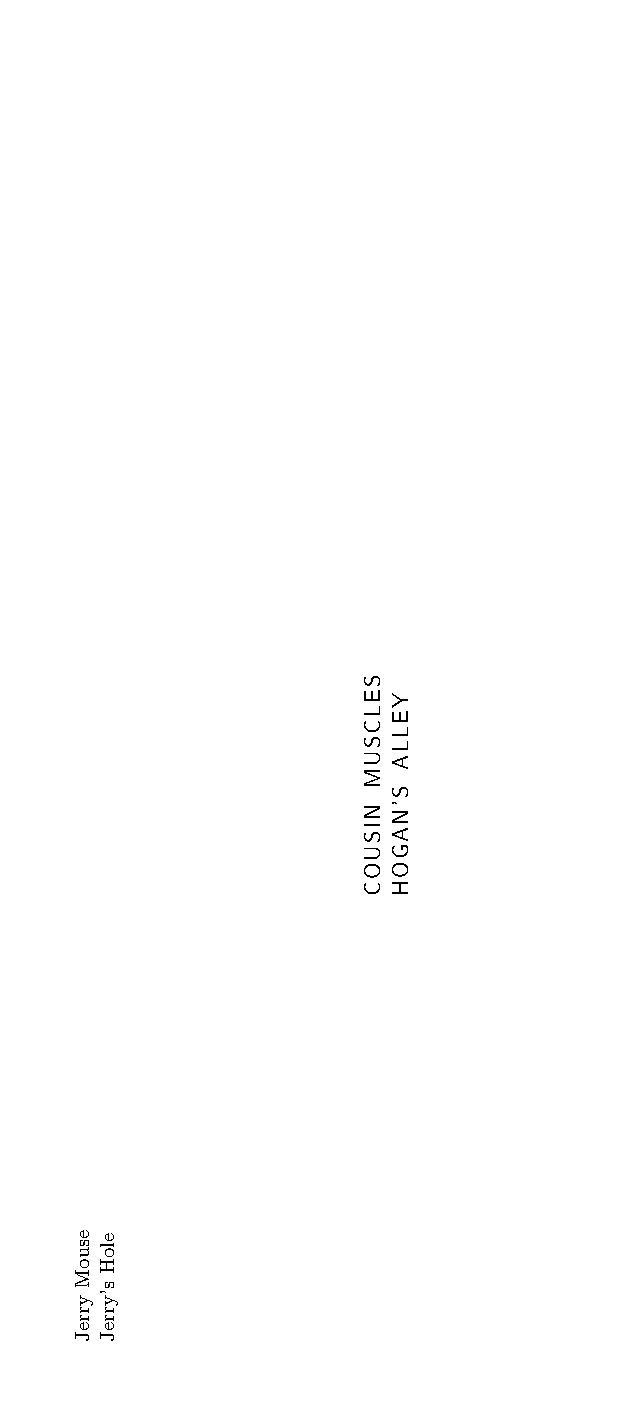
\includegraphics[scale=.5, angle=-90]{letter-env.pdf}
}
\documentclass[12pt]{letter}
\usepackage[businessenvelope]{envlab}
\usepackage[papersize={4.125in, 9.5in}]{geometry} 

\begin{document}
\startlabels
\mlabel{Jerry Mouse\\Jerry's Hole}{%
Cousin Muscles\\Hogan's Alley}
\end{document}
\end{FBTDemo}
\caption{信封}
\label{exa:letter_env}
\end{example}

\autoref{exa:letter_env} 中使用了一次 \verb|\startlabels| 命令,而另一个命令 \verb|\mlabel| 的次数根据需要而定,比如信封上只打印一次地址,制作标签时可以把多个标签放在一页内。\verb|mlabel| 命令的两个参数分别是发信人和收信人的地址。

\begin{table}[htbp]
\centering
\caption{\texttt{envlab} 宏包信封尺寸}
\label{tab:env_sizes}
\begin{tabular}{lcclcc}
    \toprule
    宏包选项          & 长度    & 高度     & 宏包选项    & 长度    & 高度\\
    \midrule
    businessenvelope  & 9.5 in  & 4.125 in & c6envelope  & 162 mm  & 114 mm\\
    executiveenvelope & 7.5 in  & 3.875 in & c65envelope & 224 mm  & 114 mm\\
    bookletenvelope   & 10.5 in & 7.5 in   & c5envelope  & 229 mm  & 162 mm\\
    personalenvelope  & 6.5     & 3.625 in & dlenvelope  & 220 mm  & 110 mm\\ 
    \bottomrule
\end{tabular}
\end{table}

\texttt{envlab} 宏包支持的信封尺寸选项见 \autoref{tab:env_sizes}。我们也可以用以下命令定制信封尺寸。 

\verb|语法:\SetEnvelope[上边距]{长度}{宽度}|

\section{简历}

在制作简历的工具中,包老师比较喜欢Xavier Danaux\indexDanaux{} \footnote{比利时天主教鲁文大学 (Catholic University of Louvain) 2006年机械硕士,法律学士。现任麦肯锡公司经理。} 的 \texttt{moderncv}。

\begin{Code}[numbers=left]
\documentclass[11pt, a4paper]{moderncv}
\moderncvstyle{casual}
\moderncvcolor{blue}
\usepackage[scale=0.8]{geometry}

\familyname{`包太雷`}
\photo[48pt][0.4pt]{picture}
\title{`雷坛巨搫`}
\quote{`一个雷人的传说`}

\address{`北京` 100081}{`白石桥路7号`}
\mobile{+86 1381-666-1643}
\phone{+86 (010) 6279-3001}
\fax{+86 (010) 6841-6688}
\email{bao@verilei.com}
\homepage{www.verilei.com}
\extrainfo{`午休时间谢绝来电`}

\begin{document}
\makecvtitle

\section{`教育背景`}
\cventry{1927--1936}{`烈士(工商管理)`}{`巴灵顿大学`}{}{}{}
\cventry{1921--1927}{`勇士(比较文学)`}{`克莱登大学`}{}{}{}
\cventry{1919--1921}{`壮士(分子生物)`}{`卧龙岗大学`}{}{}{}
\cventry{1911--1919}{`博士(有机化学)`}{`清华学堂`}{}{}{}
\cventry{1898--1900}{`硕士(天体物理)`}{`京师大学堂`}{}{}{}
\cventry{1895--1898}{`学士(应用数学)`}{`北洋大学`}{}{}{}

\section{`壮士出站报告`}
\cvitem{`题目`}{\emph{`马尾巴的功能`}}
\cvitem{`导师`}{`达文西`}
\cvitem{`摘要`}{`创造性地结合白马非马论和DNA双螺旋结构,系统性地分析`
`了马尾巴的功能。`}
\end{Code}

\begin{Code}[numbers=left, firstnumber=last]
\section{`工作经历`}
\subsection{`全职工作`}
\cventry{1936--1937}{`首席咨询顾问`}{`北美某大型财务公司`}{
`埃德蒙顿`}{}{
\begin{itemize}
    \item `调研和设计新产品:宠物意外怀孕保险`
    \item `利用业余时间引进和培训多名新员工`
    \item `按时并超额完成人寿保险推销计划`
\end{itemize}}
\cventry{1906--1911}{`高级技师`}{`欧罗巴天体实验中心`}{
`罗马`}{}{`浩瀚的宇宙,无边的探索`}
\cventry{1901--1906}{`技师`}{`希腊天体营`}{
`雅典`}{}{`摆脱束缚,解放自我`}

\subsection{`兼职工作`}
\cventry{1937--1945}{`独立董事`}{`大圣国际娱乐有限公司`}{
`温尼伯`}{}{`领衔测试新上市游戏`}
\cventry{1914--1916}{`高级实验员`}{`某餐饮连锁企业加盟店`}{
`北京`}{}{`主导研制麻辣烫高仿牛羊肉纯天然调味品`}
\cventry{1898--1899}{`图书管理员`}{`京师大学堂藏经阁`}{
`北京`}{}{`读书破万卷`}

\section{`语言`}
\cvitemwithcomment{`汉语`}{`多年来在国际著名电子公告板系统发表原创性`
`学术论文上万篇`}{`专家`}
\cvitemwithcomment{`英语`}{`大量成果登上杂志封面,并被学术带头人牛奶`
`海引用`}{`熟练`}
\cvitemwithcomment{`德语`}{`已通过德意志语言四、六级考试`}{`入门`}

\section{`电脑技术`}
\cvdoubleitem{`通用语言`}{C, C++, C\#}{`操作系统`}{
MacOS, Unix, Windows}
\cvdoubleitem{`脚本语言`}{JavaScript, Python, Ruby}{`数据库`}{
FoxPro, MySQL, Oracle}
\cvdoubleitem{`标记语言`}{HTML, \LaTeX, XML}{NoSQL}{
Cassandra, HBase, MongoDB}

\section{`荣誉称号`}
\cvlistitem{`二级中老年妇女心理咨询师`}
\cvlistitem{`崂山学者(副处级待遇)`}
\cvlistitem{`县级三好学生`}
\end{Code}

\begin{Code}[numbers=left, firstnumber=last]
\section{`业余爱好`}
\cvlistdoubleitem{`搬砖砌墙`}{`挖坑灌水`}
\cvlistdoubleitem{`割草喂猪`}{`吟诗作画`}
\end{document}
\end{Code}

\begin{example}[!h]
\begin{Demo}
\centering

\includegraphics[scale=.6, trim=0 40 0 0, clip]{cv-casual.pdf}
\end{Demo}
%\caption{简历}
%\label{exa:cv_casual}
\end{example}

\begin{example}[!h]
\begin{Demo}
\centering
\adjustbox{scale=.6, trim=0 450 0 0, clip}{
\includegraphics[page=2]{cv-casual.pdf}}
\end{Demo}
\caption{简历}
\label{exa:cv_casual}
\end{example}

这个例子比较长,包老师没找到好的排版办法,同学们凑合着看吧。在 \autoref{exa:cv_casual} 代码中,我们引入文档类后用 \verb|\moderncvstyle| 和 \verb|\moderncvcolor| 命令设置了简历的样式和颜色;还用 \texttt{geometry} 宏包设置了页边距,因为一般简历的页面都会撑得比较满。

然后,我们用 \verb|\familyname| 命令设置了姓名。因为中国人喜欢把姓放在名前面,这里没用上 \verb|\firstname| 。紧接着的照片、简历标题和摘引等,用户可根据需要有所取舍。同样地,下面的地址、电话、传真、电邮、主页等也不一定都需要。

在正文中,我们先用 \verb|\makecvtitle| 命令打印了简历标题,然后用 \verb|\section| 和 \verb|\subsection| 设置了节和小节。在教育背景一节中,我们用 \verb|\cventry| 命令列出一些学历信息,它的一般用法如下:

\verb|语法:\cventry{时间}{职位/头衔}{雇主/学校}{地点}{短说明}{长说明,另起一行}|

在出站报告一节中,我们使用了 \verb|\cvitem| 命令,它只有两个参数:

\verb|语法:\cvitem{项目标题}{说明}|

工作经历一节包含两个小节。在全职工作小节中,我们使用了通用的 \texttt{itemize} 环境;同样地,我们也可以根据需要选用 \texttt{enumerate} 环境。

在简历每页页尾,我们可以看到地址信息和页码,这些项目在其他样式中可能出现在不同位置,用户也可以自己定制。

在第二页的语言一节中,我们使用了 \verb|\cvitemwithcomment|,它比 \verb|\cvitem| 多了一个参数:

\verb|语法:\cvitemwithcomment{项目标题}{说明}{注释}|

对于比较简短的项目,我们可以像电脑技术一节那样使用 \verb|\cvdoubleitem| 命令,这样的双栏排列可以省点儿地方。

\verb|语法:\cvdoubleitem{项目标题}{说明}{项目标题}{说明}|

在荣誉称号一节,我们使用了专用的列表命令 \verb|\cvlistitem|:

\verb|语法:\cvlistitem{列表项目}|

在业余爱好一节中,我们使用了双栏列表命令 \verb|\cvlistdoubleitem|:

\verb|语法:\cvlistdoubleitem{列表项目}{列表项目}|

看完枯燥的语法,给大家来点轻松的:\autoref{exa:cv_classic} 是 \texttt{classic} 样式加绿色,\autoref{exa:cv_oldstyle} 是 \texttt{oldstyle} 样式加灰色,\autoref{exa:cv_banking} 是 \texttt{banking} 样式加橙色。它们的代码见源码包。

\begin{example}[h]
\begin{Demo}
\centering
\adjustimage{scale=.6, trim=0 420 0 0, clip}{cv-classic.pdf}
\end{Demo}
\caption{简历:古典样式}
\label{exa:cv_classic}
\end{example}

\begin{example}[h]
\begin{Demo}
\centering
\adjustimage{scale=.6, trim=0 520 0 0, clip}{cv-old.pdf}
\end{Demo}
\caption{简历:保守样式}
\label{exa:cv_oldstyle}
\end{example}

\begin{example}[!h]
\begin{Demo}
\centering
\adjustimage{scale=.6, trim=0 440 0 0, clip}{cv-banking.pdf}
\end{Demo}
\caption{简历:银行样式}
\label{exa:cv_banking}
\end{example}

在简历里,我们也可以使用普通文档中常用的一些对象,比如文献列表等。但是它们的用法没有特别的差异,所以这里就不再举例说明。

\section{棋谱}

Étienne Dupuis \indexDupuis 的 \texttt{igo} 宏包 \citep{Dupuis_2006} 可以用来排版围棋棋谱。\autoref{exa:go_bigpigmouth} 是《玄玄棋经》里的一道死活题。

\begin{example}[h]
\begin{FBTDemo}[numbers=left]{
\centering

\includegraphics[page=5]{mini.pdf}
}
\usepackage{igo}
\black{d4,f3,c4,e3,b4,f2}
\white{c3,d3,b3,e2,d1}
\black[1]{a3,a2,b1}
\copytogoban{2}
\white[4]{c2,f1}
\showgoban
\quad
\usegoban{2}
\white[4]{c1,f1,b2,d2}
\showgoban
\end{FBTDemo}
\caption{大猪嘴}
\label{exa:go_bigpigmouth}
\end{example}

代码第二、三行用 \verb|\black| 和 \verb|\white| 命令排出大猪嘴的基本形状。第四行中的命令多了个显示手数的参数,这三步棋是一本道,下面白的应法有两种。\verb|copytogoban| 命令用来保存分支前的形状。第六行是一个分支,其后的 \verb|\showgoban| 命令用来输出棋盘。\verb|\usegoban| 命令重用了之前保存的形状,第十行是另一个分支,最后一行输出另一个棋盘。

该宏包还有设置棋盘路数,棋子和字体尺寸,打印特殊符号等其他功能,感兴趣的读者可以自行查阅其手册。

\bibliographystyle{unsrtnat}
\bibliography{lnotes2}
